
\subsection*{Overall Performance}

The unregularized neural network architecture (N) was not a top performer for 
any of the six datasets. The other unregularized network, ordinary least 
squares (OLS) was the worst performer on every dataset. Ridge regression, 
a model with only L2 normalization, performed best on one dataset. 
LASSO regression, a form of L1 normalization that favors traits with few 
markers associated with moderate effects was not best on any dataset. 
Elastic Net is a regression technique that incorporates L2 and L1 
regularization together in a single model and was optimal on one dataset. 
Bayesian Ridge Regression incorporates L2 regularization, while also fitting 
regression coefficients to a Gaussian distribution. It did not perform optimally 
on any problems, but frequently performed above average. For the neural 
network family of regressors, at least one form of regularization 
outperformed the unregularized network for every dataset. Networks with 
both dropout and weight decay were able to achieve best-in-dataset 
performance on two prediction tasks. These results are summarized 
in Table \ref{tab:model-comparison}.

\ifdefined\showtablesandfigures
% Benchmark Datasets table.

\begin{table*}[htbp]
    \renewcommand{\familydefault}{\sfdefault}\normalfont
    \centering
    \caption{\bf Model Performance}

    \begin{tableminipage}{\textwidth}

        \begin{tabularx}{\textwidth}{ m{4.8em} m{4.8em} m{1.6em} m{1.6em} m{2.2em} m{1.6em} m{1.6em} m{1.6em} m{1.6em} m{1.6em} m{2.2em} }
\hline
\header & & \multicolumn{9}{c}{Accuracy} \\
\header & & OLS & RR & LASSO & EN & BRR & N & NWD & NDO & NWDDO \\
\hline
\header Species & Trait & & & & & & & & & \\
\hline
Arabidopsis & Dry Matter & 0.36 & 0.40 & 0.40 & \underline{0.42} & 0.39 & 0.38 & 0.35 & 0.39 & 0.40 \\
  & Flowering & 0.80 & 0.82 & 0.83 & 0.82 & 0.82 & 0.84 & 0.83 & 0.83 & \underline{0.86} \\
\hline
Maize & Flowering & 0.22 & 0.33 & 0.32 & 0.33 & 0.32 & 0.33 & 0.34 & \underline{0.35} & 0.33 \\
  & Grain Yield & 0.47 & \underline{0.59} & 0.49 & 0.51 & 0.57 & 0.55 & 0.52 & 0.55 & 0.51 \\
\hline
Wheat & Spike Grain Number & 0.15 & 0.27 & 0.33 & \underline{0.36} & 0.28 & 0.27 & 0.31 & 0.28 & 0.33 \\
  & Time Young Microspore & 0.59 & 0.61 & 0.74 & 0.73 & 0.64 & 0.67 & 0.74 & 0.68 & \underline{0.76} \\
\hline
\end{tabularx}

        \label{tab:model-comparison}
        \footnotesize  

        Accuracy of the best observed model performance on each dataset,
        rounded to three decimal places. The most accurate model on 
        each dataset is underlined for emphasis. 
        
    \end{tableminipage}
\end{table*}
 % Label = tab:model-comparison
\fi

Contrary to expectation, there was no consistent relationship between the 
top performing models and the species or trait evaluated, however several 
models performed notably worse than the others on all prediction tasks.
The two unregularized methods, OLS and N, as well as the L1 regularized 
LASSO were never top performers.  The BRR model also was not a top 
performer, but performed notably worse when predicting highly heritable 
traits. These results support the hypothesis that regularization is 
required to achieve optimal performance in neural network models 
and that the optimal model and regularization strategy is dependent 
on the specific species, trait, or population studied. Empirical 
validation of model accuracy is an effective way to select a 
model and regularization method for genomic prediction.

Dropout regularization tends to produce networks that have reduced 
co-adaptation of neurons \citep{srivastava2014}. For genomic prediction 
tasks, this means that haplotypes specific to only one or two 
individuals would often be included in training epochs with 
different sets of neurons enabled due to dropout regularization. Because
networks require neurons to be enabled in order to backpropagate error 
and detect patterns, more common haplotypes with consistent effects 
that persist across many different dropout iterations would be 
frequently present when particular sets of neurons are enabled and detect the
common haplotype effects instead. The detection of rare haplotypes 
that are only coincidentally and not causatively associated with 
trait performance is thus far less likely, making dropout 
regularization effective.

Weight decay is an application of L2 regularization to neural networks 
\citep{krogh1992}. Weight decay penalizes neurons with large weights values, 
allowing the backpropagation algorithm to reduce total network error by finding 
solutions with smaller weights across all inputs and interaction terms much like
ridge regression. For genomic prediction tasks, this produces models 
that perform well on traits with many predictive marker calls with small effects. 

For traits with a mixture of a few large-effect alleles and many small-effect
alleles, some combination of L1 and L2 regularization may be optimal. 
The elastic net (EN) model incorporates both of these regularization
techniques, and is the top performer on two of the six datasets presented.

While it is simple to reason about model selection for hypothetical 
genetic architectures, the architecture of a trait is rarely known prior to 
conducting a detailed analysis. To ensure that a highly accurate 
model is selected without knowledge of genetic architecture, 
we recommend evaluating a variety of models and regularization 
techniques using cross validation to identify a model that performs
well for the specific trait(s) of interest to use for making 
predictions or performing genomic selection. This eliminates 
the need to understand trait architecture in order to select an appropriate 
model.

Several models with notably high performance were not available in standard packages for
the python programming language at the time of this writing and were not included 
in this analysis. These included a family of Bayesian regression models known 
as the "Bayesian Alphabet" \citep{gianola2009} and Reproducing Kernel Hilbert 
Spaces (RKHS) regression \citep{gianola2006}.

\subsection*{Regularized Network Performance}

If a model is overfitted to training data, training data prediction accuracy is greater than 
the accuracy observed when making predictions on new datasets. Regularization methods
generally penalize models for overfitting to data. Because all measurements in this study 
were collected using five-fold cross validation sampling, models that exhibited overfitting 
should exhibit lower accuracy.

The decreased performance of the unregularized networks on several datasets in Figure 
\ref{fig:network-comparison} suggests that overfitting is sometimes a problem with 
genomic prediction applications. These results demonstrate that evaluating one 
or more regularization methods is critical to improve predictive accuracy for 
genomic prediction.

\ifdefined\showtablesandfigures

\begin{figure}[htbp]
\renewcommand{\familydefault}{\sfdefault}\normalfont
\centering 
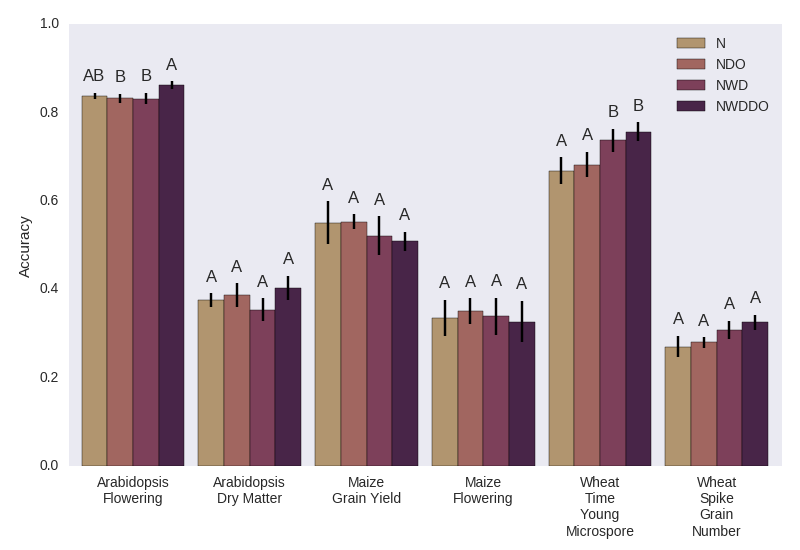
\includegraphics[width=\linewidth]{g3_article/figures/network_comparison.png}
    \caption{Predictive accuracy ($\mu \pm \sigma_{\bar{x}}$) of 
             regularized and non-regularized 
             neural network models for on benchmark datasets. Only the best performing
             network archetecture for each species, trait, and model is included. 
             The accuracy of the best performing model across all folds of data 
             and training cycles were recorded and compared. All pairwise model 
             comparisons within a species and trait were made using a two-sided paired t-test 
             (n=10, paired by training cycle and fold number).
             The resulting p-values were corrected for multiple comparisons within each 
             species and trait combination using the Holm-Bonferroni method. Columns annotated 
             with the same letter are not significantly different 
             at the $\alpha=0.05$ level.}
\label{fig:network-comparison}
\end{figure}
 % Label = fig:network-comparison
\fi

\subsection*{Deep Network Performance}

Contrary to expectation, neural networks with additional hidden layers did not perform
significantly better than networks with a single layer (Figure \ref{fig:depth-comparison}). 
One possible explanation for this observation is that by the universal approximation theorem,
sufficiently large single layer neural networks can approximate any function, including those
that deeper networks can approximate. In this study, single layer networks up to and including
those with 2187 ($3^7$) neurons were evaluated on all datasets. This number is larger than the number
of markers in any dataset evaluated and may be enough to encode complex interactions in only a single
layer.

Networks with deep architectures have proven effective on a wide variety of problems, but the largest
improvements have occurred on problems with high dimensional input data. These include voice recognition 
tasks where vocal frequencies change over a time dimension or two-dimensional images change over 
a time dimension such as in video playback. It is possible that the dimensionality of genomic 
prediction tasks tested are insufficient to benefit from the deep interaction 
effects that have proven effective in prediction tasks in other domains. 

Yet another possibility is that phenotypic measurement error on many datasets is large enough 
to mask the subtle interaction effects that would otherwise be learned by the network.

\ifdefined\showtablesandfigures

\begin{figure}[htbp]
\renewcommand{\familydefault}{\sfdefault}\normalfont
\centering 
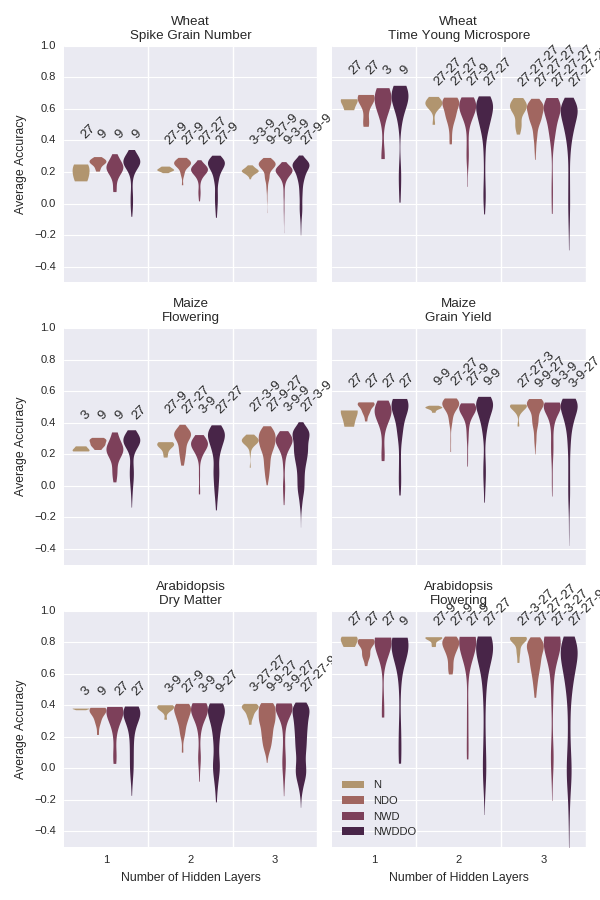
\includegraphics[keepaspectratio,height=\textheight,width=\linewidth]{g3_article/figures/depth_comparison.png}
    \caption{Distribution of predictive accuracy by benchmark dataset, network depth, 
             and model. The violin plot width indicates the Kernel Density Estimate 
             (KDE) of all observed accuracies of all models at a given network depth. 
             The sample size of the KDE is 7, 28, 28, and 112 samples for the 
             N, NWD, NDO, and NWDDO models, respectively. The models contributing 
             to each KDE vary across one or more of five weight decay, five dropout, 
             and seven hidden layer architecture parameters and can be 
             understood as the distribution of results across the set of 
             hyper-parameters to all network models with the same depth and regularization
             type. The KDE bandwidth parameters are set using Scott's normal reference rule. 
             The KDE plots are truncated to the minimum and maximum observed prediction accuracies.} 
\label{fig:depth-comparison}
\end{figure}

 % Label = fig:depth-comparison
\fi

\subsection*{GPU and CPU Training Time}

Network GPU training time was significantly different from CPU training time in all but
one genomic prediction task (Figure \ref{fig:time-comparison}). For small networks 
trained on smaller datasets such as arabidopsis, CPU training completed significantly 
faster than GPU training, though only by a small magnitude. For small networks and 
all other datasets, as well as for all large networks, GPU training time was faster 
than CPU training time on a per-core basis. These results confirm that the previously
observed speedups associated with GPU network training apply to genomic selection applications.

The time required to train a network for genomic prediction is related to
the sample size, marker count, and complexity of the network architecture to be trained.
The improvement in training time when using GPUs for model training was sub-linear across 
all three of these measures. This is because the compute capacity of modern GPUs is 
so large that the processing bottleneck is not the matrix algebra required 
to perform backpropagation but rather the speed of moving data to and from 
the memory on the GPU hardware. We frequently observed CPU utilization of 
100\% during GPU training, indicating that the GPU was demanding resources
at a rate higher than the computer system as a whole could provide them.
Consumer grade GPUs such as the NVIDIA Titan X are now available with twice 
as many CUDA cores as the GTX 680 as well a 50\% wider memory bus, making it potentially
faster than the model used for this analysis. 

It is possible to utilize additional CPU cores to linearly decrease the total time 
needed to train a network, however it is uncommon to utilize multiple GPUs for 
training the same network, and this is not supported by most software packages 
due to limitations in how memory is shared between components in systems with 
multiple GPUs. For example, a quad-core processor like the Intel i7-4790K CPU 
can train a single network approximately four times faster than indicated in 
Figure \ref{fig:time-comparison} if the entire CPU is assigned to a single
network training task. In practice, networks are trained using k-fold
cross validation, so the actual time to fit a family of networks and select
an optimal architecture would be several times larger than these values.
The growth in total time to train when using a CPU suggests that with 
networks larger than the 128x64 network in Figure \ref{fig:time-comparison}, 
CPU training time could become prohibitively large even with quad-core processors. 

Thus, choosing a network training method depends on the size of the dataset and network
to be trained. Low complexity networks train rapidly on CPUs, while larger networks
are more efficiently trained using GPUs. Cloud compute infrastructure providers such 
as Amazon Web Services (AWS) are becoming more popular, and make it much easier
to evaluate training options without purchasing expensive computer hardware.
AWS provides both CPU and GPU rich machines which can be rented at low cost 
and are charged by the hour. This makes it feasible to try CPU and GPU training
on sample data and select a training platform that is most time or cost effective based on the 
complexity of the desired network architecture and the quantity of data available
for training. 

\ifdefined\showtablesandfigures

\begin{figure}[htbp]
\renewcommand{\familydefault}{\sfdefault}\normalfont
\centering 
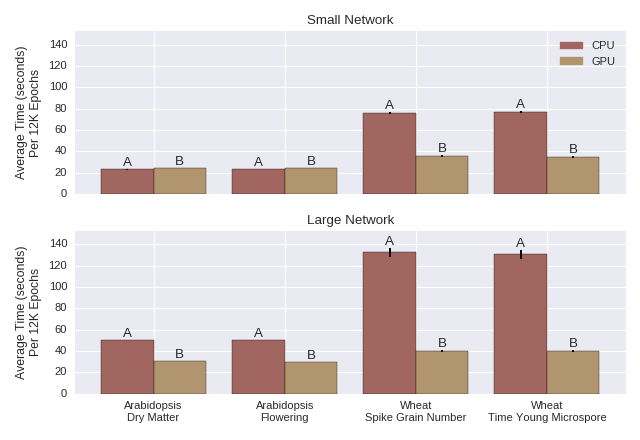
\includegraphics[keepaspectratio,width=\linewidth,height=\textheight]{g3_article/figures/time_comparison.png}
    \caption{Time to train different sized networks on identical datsets using a single dedicated CPU core
             compared to a single dedicated GPU card. Lower time to train is better. For the small network, 
             an unregularized, single hidden layer of 27 neurons was trained for 12K epochs on each dataset. 
             For the large network, two the hidden layers of size 64 and 32 neurons, respectively were trained. 
             Training processes were otherwise equal. This process was repeated ten times per dataset to 
             reduce variation associated with non-deterministic processor scheduling and varying computer system load.
             The ten CPU and GPU training samples were compared using an independent samples T-test with $n=30$. 
             CPU-GPU pairs annotated with the same letter are not significantly different 
             at the $\alpha=0.05$ level.}
\label{fig:time-comparison}
\end{figure}
 % Label = fig:time-comparison
\fi

\subsection*{Overall Conclusion}

Breeders are sometimes interested in predicting the additive genetic value of 
individuals rather than their expressed phenotype. Algorithms such as 
RKHS regression and neural networks often produce genomic prediction 
models with high predictive accuracy because they are able to capture 
interaction effects between genotypes. This is not possible with additive 
linear models such as ridge regression. As a result, caution must be exercised 
when interpreting improved prediction accuracy as a better model in the 
general case. Breeding scenarios where additive genetic value is of primary 
importance may not benefit from the use of models that capture interactions
between genes because these predictions contain non-heritable additive
variation. However, when phenotypic predictions are desirable, such 
as when breeding clonal crop varieties where individual segregates are 
selected to become commercial varieties, models incorporating interaction 
effects should perform better than models capturing only additive effects.

When combined with effective regularization techniques, neural networks can function
as accurate and effective genomic prediction models with a low risk of overfitting
to training data. With the ready availability of GPU computation resources, concerns
over total time to train are partially ameliorated. Searches for optimal architectures or 
regularization techniques can be automated in a time and cost effective 
manner using cloud compute providers such as AWS.

